

\documentclass[fontsize=12pt]{article}
\usepackage{fourier}
%%% Custom sectioning
\usepackage{sectsty}
\allsectionsfont{\flushleft \normalfont\scshape}

\usepackage[english]{babel}															% English language/hyphenation
\usepackage[protrusion=true,expansion=true]{microtype}	
\usepackage{amsmath,amsfonts,amsthm} % Math packages
\usepackage[pdftex]{graphicx}	

\usepackage{url}
\usepackage[margin=1 in]{geometry}
\geometry{a4paper}

\usepackage{graphicx}
\usepackage{listings}
\usepackage{float}
\usepackage{xcolor}
% page counting, header/footer
\usepackage{fancyhdr}
\usepackage{lastpage}
\pagestyle{fancy}
\lhead{\footnotesize \parbox{11cm}{Office Object Recognition} }
%\renewcommand{\headheight}{24pt}


\begin{document}

\begin{titlepage}

\newcommand{\HRule}{\rule{\linewidth}{0.5mm}} % Defines a new command for the horizontal lines, change thickness here

\center % Center everything on the page
 
%----------------------------------------------------------------------------------------
%	HEADING SECTIONS
%----------------------------------------------------------------------------------------

\textsc{\LARGE Erasmus Mundus Master in Vision and Robotics}\\[1.5cm] % Name of your university/college
\textsc{\Large B31XP:Robotics Project }\\[0.5cm] % Major heading such as course name
%\textsc{\large Minor Heading}\\[0.5cm] % Minor heading such as course title

%----------------------------------------------------------------------------------------
%	TITLE SECTION
%----------------------------------------------------------------------------------------

\HRule \\[0.4cm]
{ \huge \bfseries Office Object Recognition}\\[0.4cm] % Title of your document
\HRule \\[1.5cm]
 
%----------------------------------------------------------------------------------------
%	AUTHOR SECTION
%----------------------------------------------------------------------------------------

\begin{minipage}{0.4\textwidth}
\begin{flushleft} \large
\emph{Los Lobos Solitarios v2.0}\\
Abraham \textsc{Ayala} \\% Your name
Quim \textsc{Sanchez}\\ % Your name
Waldemar \textsc{Franczak}\\ % Your name
\end{flushleft}
\end{minipage}
~
\begin{minipage}{0.4\textwidth}
\begin{flushright} \large
\emph{Supervisor:} \\
Dr. Zeyn \textsc{Saigol} % Supervisor's Name
\end{flushright}
\end{minipage}\\[4cm]

% If you don't want a supervisor, uncomment the two lines below and remove the section above
%\Large \emph{Author:}\\
%John \textsc{Smith}\\[3cm] % Your name

%----------------------------------------------------------------------------------------
%	DATE SECTION
%----------------------------------------------------------------------------------------

{\large \today}\\[3cm] % Date, change the \today to a set date if you want to be precise

%----------------------------------------------------------------------------------------
%	LOGO SECTION
%----------------------------------------------------------------------------------------

%\includegraphics{Logo}\\[1cm] % Include a department/university logo - this will require the graphicx package
 
%----------------------------------------------------------------------------------------

\vfill % Fill the rest of the page with whitespace

\end{titlepage}
\tableofcontents
\pagebreak[4]
\section{Introduction}\label{sec:intro}
During this report it will be described the advances done by Lobos Solitarios v 2.0 team in the Office Object Recognition project. The general goal of the project is to implement a pipeline which provides the ability to a mobile robot of performing object recognition of commonly present objects in an office environment.This information will give some insight to the robot about its environment, and will help it to perform more advanced and useful tasks. 
This work is organized as follows, in section \ref{sec:probdesc} the problem description and previous work will be explained. In sections  \ref{sec:pplanning} and \ref{sec:toolseval} is documented the project planning and learning process to propose a solution. In sections \ref{sec:map},\ref{sec:planeseg},\ref{sec:clustering} and \ref{sec:recognition} is explained the proposed solution of the team in this starting point of the project. Finally in section \ref{sec:Future Work} and \ref{sec:Conclusions} is settled the future work to be done and the conclusions about the work done.  
\section{Problem description and Previous work} 
\label{sec:probdesc}
Preferably the system should be able to recognize the common office objects even though the object is partially occluded or only part of its components are seen, to achieve this a possible solution is to define object classes which are composed by different elements. For example a chair is composed by different elements as shown in figure \ref{fig:chair}, in some situations is possible that the robot only observes one or several of this subcomponents of the class chair. The system should be able to recognize or give probabilities of how likely is a set of structural elements to form an object class.
\begin{figure}[H]
\begin{center}
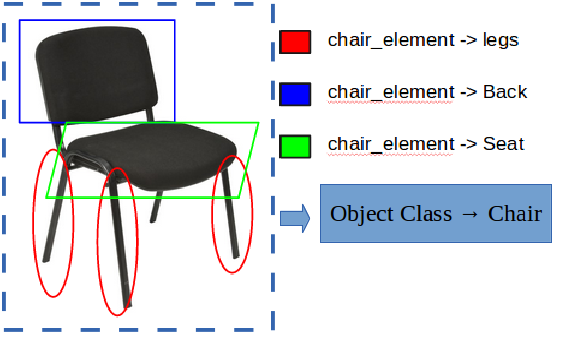
\includegraphics[width=0.5\linewidth]{images/chair}
\caption{Decomposition of the class 'chair' into its structural elements}
\label{fig:chair}
\end{center}
\end{figure}
In a more advanced phase of the project, is intended to provide the robot the ability to identify when an object is incomplete, this with the purpose of moving the robot to the unknown part of the object and fuse the information of different views. 
The whole project of object recognition is intended to be realized by several VIBOT generations, and for the case of this semester the goal is to propose a starting point for the problem. 

The available hardware platform for this starting point is:
\begin{itemize}
\item Turtlebot 2 mobile robot from willow garage and clearpath
\item Microsoft Kinect (640x480) RGB-D camera integrated in turtlebot
\end{itemize}
In terms of software framework, the desired or preferable platforms to develop the project are:
\begin{itemize}
\item ROS (Robot Operating System) from willow garage
\item ORK (Object Recognition Kitchen)\cite{bib:ORK}
\end{itemize}
One important requirement to follow is the integration of the proposed pipeline with ROS, since turtlebot robot is optimized to be controlled by ROS.
About previous work realized, in \cite{bib:semantic} is described a general approach using ORK pipeline, manual labelling and 3D data registration to train different types of office objects to fuse and segment them in different views.  \linebreak
A initial requirement of the supervisor of this project is to try to solve the application using of-the-shelf algorithms of OpenCV \cite{bib:OCV} provided by the object recognition framework, following the work done in \cite{bib:semantic}.
\section{Project Planning}
\label{sec:pplanning}
The initial gant diagram of the project was planned to follow the milestones shown in figure \ref{fig:plan1}, in which the first two weeks were intended to determine if the ORK framework could provide the necessary software tools to develop the application.
\begin{figure}[H]
\begin{center}
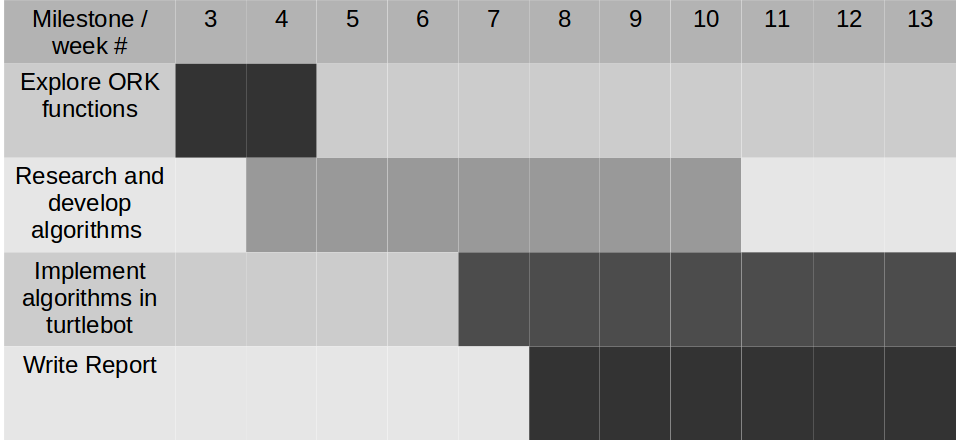
\includegraphics[width=0.8\linewidth]{images/plan1}
\caption{Lobos Solitarios gant diagram}
\label{fig:plan1}
\end{center}
\end{figure}

\section{Tools selection and evaluation}
\label{sec:toolseval}

Explanation of ORK and the work done in ORK, justification on why was not used the ORK and why PCL is a useful solution
\subsection{Project Reconsideration}
\label{sec:projreco}
Description of the new planning and the splitting of the tasks between the team members,as well the general pipeline to follow to achieve a first approach to the problem with the pcl tools
\section{3D mapping}
\label{sec:map}
As explained in section \ref{sec:probdesc}, and the new requirement of the supervisor to perform the 3D mapping in this first part of the project, The robot should be able to build a 3D map of the places it has visited, for later use to detect the objects and identify their position in the map. The next possible solutions to register point clouds or build the 3D representation of the readings of the robot were analysed:
\begin{itemize}
\item CCNY visual odometry and 3D map building
\item PCL point cloud registration
\item octomap 3D mapping
\end{itemize}

\subsection{CCNY visaul odometry}
Explain about this method
\subsection{Point cloud registration using PCL}
Explain

The \textit{pcl } library has some methods to perform point cloud registration, which are iterative process that aligned two given point clouds.
 \linebreak

\subsection{Octomap 3D mapping}
Based in octrees, several depths or resolutions can be queried
Each node saves the probability to be occupied or free (helps to handle noise)
Map build incrementally , known and unknown areas available.
\begin{figure}[H]
\begin{center}
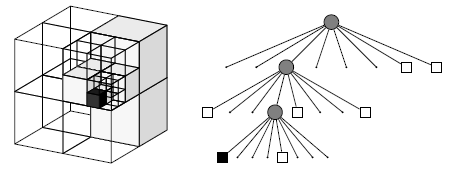
\includegraphics[width=0.8\linewidth]{images/octree}
\caption{Octree representation}
\label{fig:octree}
\end{center}
\end{figure}

\begin{figure}[H]
\begin{center}
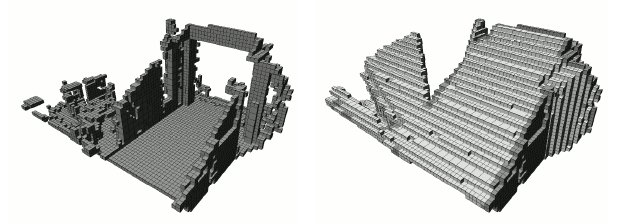
\includegraphics[width=0.8\linewidth]{images/octofree}
\caption{In the left the representation of occupied voxels, in right the representation of free and occupied voxels}
\label{fig:octreefree}
\end{center}
\end{figure}

\begin{figure}[H]
\begin{center}
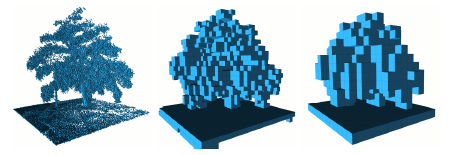
\includegraphics[width=0.8\linewidth]{images/treedifres}
\caption{Different resolutions of the octomap}
\label{fig:difrefocto}
\end{center}
\end{figure}

\begin{figure}[H]
\begin{center}
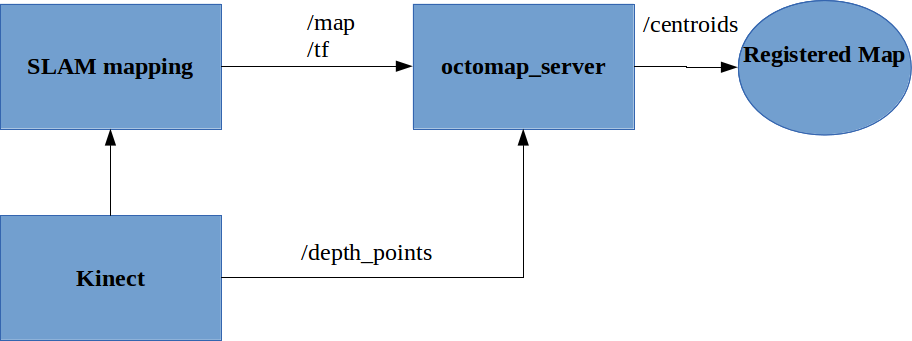
\includegraphics[width=0.8\linewidth]{images/diagocto}
\caption{Octomap integation with ROS}
\label{fig:OctowithROS}
\end{center}
\end{figure}

\begin{figure}[H]
\begin{center}
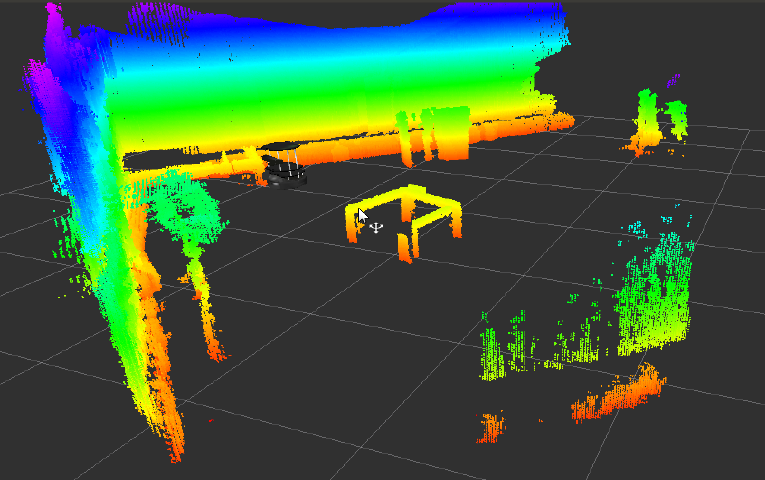
\includegraphics[width=0.8\linewidth]{images/figoctomap}
\caption{Octomap 3D mapping of a scene}
\label{fig:octoscene}
\end{center}
\end{figure}





\section{Plane Segmentation}
\label{sec:planeseg}

To make the search of primitives easier we first decided to segment the date following some rule that would make smaller set but at the same time would not split the objects. After doing some literature review we found this paper were they propose a method to detect and segment planes in a fast way. The main contribution from this paper is the idea of using the range image neighbourhood information to proximate the real point neighbour. Then they propose some simple ways to cluster the data as well.\\

\subsection{Algorithm outline}

The algorithm consists of 3 main parts:

\begin{itemize}
  \item Normals computation
  \item Normals clustering
  \item Parallel planes distinction
\end{itemize}

\subsubsection{Normals Computations}

One way to represent planes is by its normal and one point belonging to the plane. To conclude it two points belong to the same plane we need to compute the Normal vector in each of the points.  To compute the Normal of one point the information of its neighbours is needed and so  the first problems is, how can we find the neighbour of a point? One approach is to use the closest points using KNN and some fast implementation. Once this points are found a plane can be fit and from it calculate its normal.\\

The problem of this approach is that the search of neighbours can be very computationally expensive even when using fast algorithm that only approximate the result. Also, if many points are fit to the plane, the computation of the normal vector using eigen decomposition can also be expensive. \\

In the proposed method both steps are substituted by much simpler and faster operations.\\

First of all the algorithm assumes that two pixels in the range image will still be neighbours once they are projected in the 3D space. This will not hold on the edges of planes but in general it can be accepted. At this step the algorithm computes two tangential vectors of the point using the difference between the points of right and left pixel for the horizontal and above and bellow pixel for the vertical. Then it computes the cross product of this two tangential vectors to compute the normal.\\


\subsubsection{Normals Clustering}

After on normal is computed for each of the points a second step comes which will cluster similar normals with the idea that they will belong to the same plane. To do the clustering different iterative algorithm like k-means could be used but to avoid computation a different method is used. In this case an octree is build with the normals as points, this way similar normals will fall in the same octree voxel. Initially each voxel with data will be a different plane.\\

The performance of this method is very sensitive to the size chosen for the voxels. Too large voxels will not be able to distinguish between similar plans and too small voxels will oversegment the planes. This problems are partially attenuated with two methods, this first one is to smooth the normals using again the range image neighbourhood idea. Every component of the tangential vectors ($XYZ$) is set up as an image with the same shape as the range image and a Gaussian filter is applied to it. This makes the normals more homogeneous removing small changes.\\

A second method is to compare the clustered planes by their mean and to merge them if we decide that they are very similar. This also solves the problem of one plane cluster falling between two voxels.\\ 

\subsubsection{Parallel planes distinction}

So far the algorithm is  able to distinguish between planes with different normals but parallel plans share a normal while not being the same plane. During this third step this differentiation is carried out.\\


The feature used to distinguish between points of different parallel planes is to calculate the distance from the point to the plane deffined by the mean normal and a given point, usually (0,0,0). Points from the same plane will have the same distance to this reference plane.\\

Finally to cluster this distances the same technique from the previous step is used.\\

\section{Point Cloud Clustering}
\label{sec:clustering}
\section{Object Recognition}
\label{sec:recognition}
\section{Future Work}
\label{sec:Future Work}
\section{Conclusions}
\label{sec:Conclusions}

\begin{thebibliography}{9}

\bibitem{bib:semantic}
  Jorg Stuckler, Nenad Biresev, and Sven Behnke
  \emph{ Semantic Mapping Using Object-Class
Segmentation of RGB-D Images}.
  In Proc. of the IEEE/RSJ Int. Conf. on Intelligent Robots and Systems (IROS), Vilamoura, Portugal, October 2012 (corrected).
  \bibitem{bib:ORK}
  Willow garage. 
  \emph{Object recognition kitchen}. 
  \url{http://wg-perception.github.io/object_recognition_core/}
  \bibitem{bib:OCV}
  OpenCVorg.\emph{Open Source Computer Vision Library}
  \url{http://opencv.org/}
\end{thebibliography}
\end{document}